\documentclass[hyperref,UTF8]{ctexart}
\usepackage[dvipdfmx]{graphicx}
\usepackage{gbt7714}
\usepackage{float}
\usepackage{ragged2e}
\usepackage{amsthm}
\usepackage{amssymb}
\usepackage{amsmath}
\usepackage{wrapfig}
\usepackage{tikz}
\usetikzlibrary{arrows.meta}
\usepackage{booktabs}
%\usepackage[a4paper,left=3.18cm,right=3.18cm,top=2.54cm,bottom=2.54cm]{geometry}
\usepackage{tabularx}
\usepackage{array}
\usepackage{caption}
\usepackage{hyperref}
\newcommand{\upcite}[1]{\textsuperscript{\textsuperscript{\cite{#1}}}}
\setCJKfamilyfont{song}{SimSun}
\newcommand{\D}{\mathrm{d}}
\title{讲义}
\author{limbo137}
\begin{document}
\maketitle
\part{力学}
\section{运动学}
运动学是物理理论中最“实在”的一部分,我们完全可以找除牛顿力学以外另一种物理理论来描述我们的世界,但这个理论正确与否,也要靠其造成的运动学“实在”来验证。如果同样情况下两种物体做不同的运动,那么显然有一种理论出了问题。

我们通常所说的运动,实际上指的是物体的“运动状态”随时间的变化,这便是整个运动,\textbf{运动状态其实就是质点的速度矢量},那么整个运动就是速度矢量随时间变化的函数
\[\vec{v}(t)\]
为什么说知道这个就知道整个运动了呢,因为由速度函数可以通过求导求出加速度函数$\vec{a}(t)$,而位移函数$\vec{x}(t)$也可以通过反推得到,下面我们举直线运动的例子来说明这一点。
\subsection{直线运动}
在直线运动中,原来的矢量变成了标量,于是速度,加速度,位移三者之间的关系也变得简单了起来
\begin{align*}
    a &= \frac{\D v}{\D t} \\
    v &= \frac{\D x}{\D t}
\end{align*}
根据导函数和原函数的定义\footnote{参见数学选修2-2},我们也可以得到$v-t$图上,加速度和位移的几何意义,就是切线斜率和面积,
%此处有一个斜率和面积的图

一类最特殊也最常考的运动就是匀加速直线运动,这类运动的核心是加速度不变,我们从数学上可以算出$v$和$x$
\begin{align*}
    a &= \frac{\D v}{\D t} \\
    v &= \frac{\D x}{\D t} =a t + v_0\\
    x &= v_0 t + \frac12 a t^2
\end{align*}
整理一下,下面这两个方程就是匀加速直线运动的基本方程了,从理论上来讲,一切关于匀加速直线运动的问题都可以利用这两个方程解决
\begin{equation}
    \begin{split}
        v &=a t + v_0\\
        x &= v_0 t + \frac12 a t^2
    \end{split}
\end{equation}
为了方便,我们还需要$x$与$v$的关系,这个时候上面两式约掉$t$
\begin{equation}
    v^2-v_0^2=2ax
\end{equation}
\textbf{匀加速直线运动中的二级结论}

在相等的时间间隔下,匀加速直线运动的位移
\subsection{曲线运动}
\subsection{圆周运动}
处理圆周的问题离不开角度,不过这里的角度要换成弧度制,它定义成弧长与半径之比,
\[
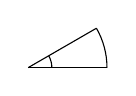
\begin{tikzpicture}
    \draw (0,0)--(0:1);
    \draw (0:1) arc [start angle=0, end angle=30, radius=1cm];
    \draw (3mm,0mm) arc [start angle=0, end angle=30, radius=3mm];
    
    \draw (0,0)--(30:1);
\end{tikzpicture}
\]
\[v = \omega r\]
\begin{align*}
    a &= v\omega\\
    & = {v^2 \over r}\\
    & = \omega^2 r
\end{align*}
抛体运动
\begin{align*}
    x &=v_x t \\
    y &=v_y t - \frac12 gt^2  
\end{align*}
\[y = x \tan\theta -{gx^2 \over 2v\cos^2{\theta}}\]
一般的曲线运动
\[a = {v^2\over \rho }\]
其中$\rho$称为\textbf{曲率半径}
\section{动力学}
\subsection{牛顿定律}
牛顿第二定律(力的定义)
\[F = ma\]

弹力
\[F(x) = -kx\]

滑动摩擦
\[f=\mu N\]

万有引力
\[F(r) = {GMm \over r^2}\]

重力
\[G = mg\]

\section{静力学}
静摩擦
\[F_{\text{静}}=F_{\text{外}}\]

沿杆,绳方向的力的判断
\subsection*{受力分析综合}
受力分析的几个步骤

1.找好方向,做好投影

2.判断运动状态,合外力等于$ma$(注意方向)

3.解方程,求出所求力或加速度
\section{机械能}
\subsection{动能和动能定理}
\textbf{动能定理}:合外力做功等于动能的变化\\
对于受恒定力的质点
\begin{align*}
    \Delta E_k &= Fx \\
    &=max \\ 
    &=\frac12 m(v^2-v_0^2)
\end{align*}
于是动能定义为
\[E_k = \frac12 mv^2\]
\subsection{势能}
\[\D E_k = F \D x\]
如果可以定义\footnote{很多时候,我们无法找到这样的$E_p$使这个定义成立,这样的外力场称为非保守的,此时的势能要用另外的方式定义或无法定义}
\[-\D E_p = F \D x\]
这个$E_p$就称为势能\\则有
\[\D (E_k+E_p) = 0\]
这说明,动能加势能的和是一个在运动中不变的量,我们称之为\textbf{守恒量}\\
那么我们得到了另外一个力的定义
\[F = -\frac{\D E_p}{\D x}\]
我们对这两种定义进行一些评述,在粒子(质点)在外力场的作用下,第一种定义中的$m$是物体本身的属性,表示对外力的一种“抵抗”,也就是物体本身的惯性,而加速度$a$则是粒子对外力场的一种“响应”。而第二种定义中势能是外力场的性质,势能的对空间的导数表明了势能的局部性质,表示对粒子的一种“作用”,或者叫“扰动”,可以说第一种定义是粒子是如何对作用进行响应的,而第二种定义则是说明了外场是如何对粒子进行扰动的,所以我们联立两式,消去$F$
\[-\frac{\D E_p}{\D x} = ma\]
这个结果是分析力学拉格朗日方程的变体,中如果我们只看这种响应的结果$a$
\[a = -\frac{\D E_p}{m\D x}\]
可以看出,质量$m$是一种对外场的“抵抗”
\subsection{动量}
在两个物体的相互作用中,还有其他的守恒量

考虑两个互相作用的物体,除此之外没有其它作用,我们有牛顿第三定律
\[\vec{F}_{12} = - \vec{F}_{21}\]
12表示物体1对物体2的作用,21反之,负号表示方向相反,我们利用牛顿第二定律
\[m_1\frac{\D \vec{v}_1}{\D t}=-m_2\frac{\D \vec{v}_2}{\D t}\]
移项可以得到
\[\frac{\D }{\D t}(m_1\vec{v}_1+m_2\vec{v}_2)=0\]
定义总动量为$\vec{p}$
\[\vec{p} = m_1\vec{v}_1+m_2\vec{v}_2\]
\section{万有引力和天体}
\subsection{从万有引力到开普勒三定律}
万有引力定律写成
\[F(r) = {GMm \over r^2}\]
要想得到加速度,要与$F=ma$结合,我们有
\[a(r) = {GM \over r^2}\]
这个关系是天体中最本质的关系,也是卫星运动的基本方程,注意这个加速度指向中心天体,我们想到如果这个天体的速度的大小和方向合适,那么可以做圆周运动,什么是合适的大小和方向?先让上面这个加速度等于圆周运动的向心加速度
\[{v^2 \over r} = {GM \over r^2}\]
可以解出
\[v = \sqrt{\frac{GM}{r}}\]
也就是说,当一个质点在$r$处时,必须以垂直于质点-天体连线为方向,以$\sqrt{\frac{GM}{r}}$为初速度大小发射时,质点\textbf{才能}做圆轨道运动,可见这种条件是十分苛刻的。好在,在我们的太阳系中,几大行星的轨道都十分接近正圆形。\\
\[
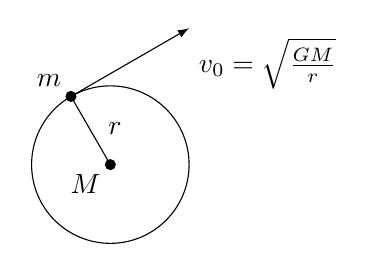
\begin{tikzpicture}
    \draw (0,0) circle (1cm);
    \fill (120:1) circle (2pt);
    \fill (0,0) circle (2pt);
    \node[below left] (O) at (0,0) {$M$};
    \node[above left] (A) at (120:1) {$m$};
    \node[below right] (A) at (60:2) {$v_0 = \sqrt{\frac{GM}{r}}$};
    \draw[-latex] (120:1)--(60:2);
    \draw (0,0)--(120:1);
    \node[above right] (O) at (120:0.3) {$r$};
\end{tikzpicture}
\]
\textbf{什么决定了天体的轨道?}

把一个质点在一个天体附近以一个初速度射出,那么它的轨道就是既定的,既然如此,就是先知道了初速度$v_0$和距离$r$,那么我们就不应该不分青红皂白的写向心力方程,我们应该沿着物理学基本的寻找守恒量的观点,
去寻找质点在只收万有引力作用下的守恒量,这个量可以从数学上推导出来,人们发现,在一个只受有心力\footnote{不止是万有引力,凡是受力方向始终指向一点均可}的系统中,下面的量是守恒的($v_\theta$是垂直于受力方向的速度分量,称为切向速度)
\[v_{\theta}r = {r^2\Delta \theta \over \Delta t} = {\Delta S \over \Delta t}\]
即单位时间扫过的面积,我们称之为掠面速度,掠面速度守恒就是开普勒第二定律的主要内容。
\begin{figure}[H]
    \centering
    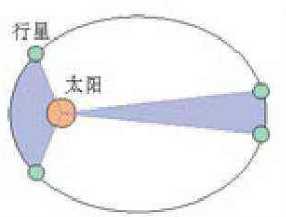
\includegraphics[width=3cm]{掠面速度.png}
    \caption{行星与太阳的连线在相等的时间扫过相等的面积}
\end{figure}
通过掠面速度守恒和万有引力定律,我们可以得出行星的轨道是一个椭圆,中心天体处在这个椭圆的一个焦点上,即开普勒第一定律,想要证明这一点并非易事,Feynman曾有一个巧妙的证明\footnote{参见\url{https://www.bilibili.com/video/BV1Zs411A7KJ?from=search&seid=6802919749265632960}},我们这里不过多介绍。

我们来对绕天体做半径为$R$圆轨道的卫星的周期做一些推导,周期$T$满足
\[T^2 = (\frac{2\pi R}{v})^2=\frac{4\pi^2 R^3}{GM}\]
于是
\[\frac{T^2}{ R^3} = \frac{4\pi^2}{GM}\]
在椭圆轨道中也有类似的结果,不过需要把$R$换成半长轴$a$
\[\frac{T^2}{a^3} = \frac{4\pi^2}{GM}\]
这就是开普勒第三定律,半长轴的三次方和周期的二次方成正比,由表达式还可看出,这个比值只于中心天体的质量有关。这个也是一个守恒量,不过要在多个卫星绕同一天体运行时才起作用,上面的掠面速度守恒则适用同一卫星运行时的不同位置时。

\subsection{宇宙速度}
我们在地球上抛出一个物体时,它做什么轨道运动,我们学过抛体运动,知道它将做抛物线运动,但是事实果真如此吗?抛出的苹果和天上的月亮会出现不同的轨道吗?

事实上,无论是抛出的苹果,还是天上的月亮,都在做椭圆轨道运动,只不过抛出的苹果速度太小,椭圆的半长轴太大(要想到另外一个焦点是地球中心),这个椭圆是如此之扁以至于它无论如何都会返回地面,而这一小部分运动轨迹就看起来像抛物线一样(图中这个椭圆还不够扁)
\[
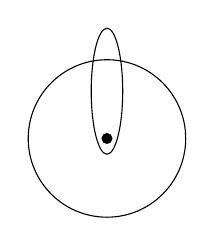
\begin{tikzpicture}
    \draw (0,0) circle (1cm);
    \draw (0,0.6) ellipse (0.2cm and 0.8cm);
    \fill (0,0) circle (2pt);
    \node[below left] (O) at (0,0) {};
\end{tikzpicture}
\]
所以,如果在地球附近沿切线射出一个物体,不考虑其它因素,如果速度合适,那么这个物体就可以绕地球(在地表附近)做圆轨道运动,这个速度也是发射卫星的最小速度,我们让上面的圆轨道条件中的$r$替换成地球半径$R$,我们得到了这个速度
\[v_1 = \sqrt{\frac{GM}{R}}=7.9 \mathrm{km}/\mathrm{s}\]
称为\textbf{第一宇宙速度}

那么既然能在地球附近做轨道运动,我们在航天上更关心,它速度达到多大时,可以脱离地球引力的束缚,这时就有了\textbf{第二宇宙速度}

为了介绍第二宇宙速度,我们先给出引力势能的概念\footnote{这部分仅作了解},引力势能与电势能类似,在无穷远初为0,越靠近中心天体越小,所以正常情况下这个势能为负
\[E_p = -\frac{GMm}{r}\]
其中$r$是到中心天体中心的距离,那么根据机械能守恒,我们出发点在地球表面,初速度是$v_0$,总能量是
\[\frac12 mv^2_0-\frac{GMm}{R}\]
在逃离中心引力场的束缚时,动能不断变为引力势能,如果将全部动能用完也还没能抵消完全势能,那么就无法脱离引力的魔爪,但要是引力势能变为0时(即无穷远),动能还有剩余,此时的总能量大于0,那么就是成功脱离了引力的束缚,于是我们只需要让总能量大于0,就是脱离的条件,即
\[\frac12 mv^2_0-\frac{GMm}{R} \geqslant   0 \]
解得
\[v_0\geqslant \sqrt{\frac{2GM}{R}}\]
右边的速度就是最小速度,即第二宇宙速度,也叫逃逸速度
\[v_2 = \sqrt{\frac{2GM}{R}} = 11.2 \mathrm{km}/\mathrm{s}\]

脱离太阳的引力要复杂的多,这里径直给出结论
\[v_3 = 16.7\mathrm{km}/\mathrm{s}\]
\subsection{引力半径和黑洞}
由逃逸速度的表达式可知,恒星质量越大,半径越小,逃逸速度越大,我们知道宇宙中的速度极限是光速,那么有没有逃逸速度是光速的天体呢?我们来推导一下这种天体应该满足的条件
\[v_2= c = \sqrt{\frac{2GM}{R}}\]
于是
\[R = \frac{2GM}{c^2}\]
这个半径称为\textbf{施瓦西半径},也叫引力半径,天体半径小于这个半径的天体叫\textbf{黑洞}
\section{振动与波*}

\part{电磁学}
\section{静电场}
\section{稳恒电流}
\section{磁场}
\section{电磁感应}
\section{交流电}
\part{热学*}
\section{微观理论}
\section{宏观理论}
\part{光学*}
\section{几何光学}
\section{波动光学}
\part{近代物理}
\section{原子物理}
\section{相对论初步}
\end{document}